\chapter{Introdução}

\section{Apresentação}

Reconhecimento de gestos baseado em visão computacional é um assunto bastante pesquisado e já pode ser considerado popular, isto porque, a busca por mecanismos que tornem a interação entre homem e máquina mais intuitiva e natural é constante e vem aumentando com o lançamento de plataformas que auxiliam os desenvolvedores nos complexos algoritmos que envolvem essa área.
O lançamento do Kinect, da Microsoft \cite{kinect}, e da plataforma de desenvolvimento da Intel, chamada Intel Perceptual Computing \cite{intel} (figura \ref{fig:depth_camera}),  ambas com câmeras de profundidade, vem popularizando o desenvolvimento de aplicativos e revolucionando o jeito que interagimos com os jogos e computadores. 

\begin{figure}[ht!]
\centering
\fbox{
  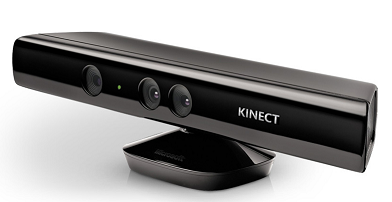
\includegraphics[width=0.3\textwidth]{image/kinect_camera.png}
  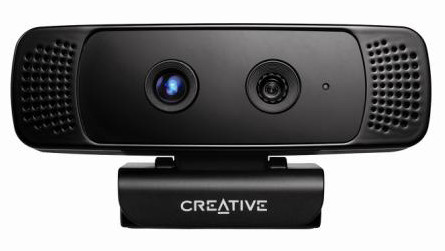
\includegraphics[width=0.3\textwidth]{image/intel_creative_camera.jpg}}
  \caption{Kinect, da Microsoft, e a câmera da \textit{Creative} com parceria da Intel}
  \label{fig:depth_camera}
\end{figure}

O uso de câmeras em carros e caminhões também tem aumentando nos últimos anos. Sistemas de segurança capazes de verificar se o motorista esta saindo indevidamente da faixa, ou se o veículo esta em rota de colisão com algum outro automóvel ou objeto e até mesmo monitorando o stress do motorista já são comuns em vários modelos de veículos. Mas pouco vimos o uso dessas câmeras para interação do motorista com a grande quantidade de controles que temos nos carros. Sistemas de navegação, componentes de som e imagem como CD/DVD player, radio, televisão, celulares, computador de bordo, e ar condicionado são alguns exemplos de dispositivos que requerer uma constante interação com o motorista e cujo comandos poderiam ser dados por meio de gestos.
O sistema de gestos também pode ser usado como um complemento ao sistema de reconhecimento de voz, bastante comum hoje nos carros.

Nesse sistema gestual de interação do motorista com o veículo, podemos entender poses e gestos como sendo movimentos ou poses executados pela mão direta do motorista dentro do campo de visão de uma câmera instalada no teto do carro.
O nosso estudo, portanto, é focado no histograma orientado a gradientes (HOG - Histogram of oriented gradients) aplicado em um sistema de interface de usuário através de gestos. Um sistema em tempo real capaz de reconhecer poses de mão e gestos que permita o motorista interagir com o veículo de forma intuitiva e eficaz. Na figura \ref{fig:visao_aplicacao} temos um exemplo de como seria uma pose de mão aberta dentro de um ambiente automotivo.

\begin{figure}[ht!]
\centering
\fbox{
  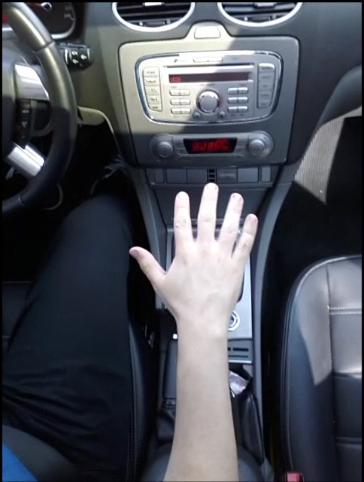
\includegraphics[width=0.3\textwidth]{image/exemplo_visao_aplicacao.png}}
  \caption{Exemplo do uso de poses em um ambiente automotivo}
  \label{fig:visao_aplicacao}
\end{figure}

\section{Objetivo}

Um dos primeiros passos no processamento de uma imagem, com o objetivo de se identificar uma pose, seria encontrar a região de interesse. Essa região é uma sub-imagem onde a mão aparece com mais evidencia, eliminando as partes que não são de interesse. A partir dai os mais diversos algoritmos podem ser aplicados para se identificar a pose.
O objetivo do trabalho é encontrar essa região de interesse utilizando o HOG. HOG é um conjunto de técnicas que usam a orientação da variação das bordas para caracterizar a imagem. Uma grande vantagem dessa técnica e sua grande robustez contra variações de luminosidade. A proposta é portanto estudar o efeito da variação dos principais parâmetros do cálculo do HOG e assim encontrar qual a melhor configuração para a aplicação proposta. Um balanço entre performance e processamento deve ser levado em consideração, já que o trabalho computacional deve ser reduzido ao máximo para aplicações automotivas.

O HOG foi proposto por Dalal em 2005\cite{dalal} que encontrou o melhor conjunto de parâmetros para a representação de seres humanos em diversas situações e poses diferentes. O que queremos avaliar é se para a nossa aplicação, os mesmos parâmetros podem ser aplicados e qual seria o custo na performance do algoritmo se o mesmo fosse simplificado com o intuito de reduzir processamento.
O HOG poderia ser usado de duas maneiras diferentes: como um pre classificador para encontrar as regiões mais prováveis de se ter uma mão e assim limitar a imagem em algumas regiões de interesse aonde um segundo algoritmo seria aplicado, nesse caso não seria trabalho do HOG dizer qual é a pose, mas sim se é uma mão ou não, ou no máximo classificar a pose em algum grupo de poses (como feito em \cite{ref10}). Mas o HOG poderia ser usado também para dizer qual pose é, sem a necessidade de nenhum algoritmo secundário.
Visando que temos duas aplicações para o HOG, é possível que teremos duas configurações diferentes e portanto essas variações devem entrar no escopo desse trabalho.

\section{Justificativa}

A função principal do motorista deve ser sempre o controle do veículo. Distrações, como operar o rádio ou a central multimédia são exemplos constantes de cause de acidentes. Portanto apenas alguns poucos e curtos momentos podem ser usados para interagir com os comandos do veículo. Em estudos de usabilidade, o controle gestual provou ser mais intuitivo, efetivo \cite{ref12}  \cite{ref13} e distrair menos do que o uso habitual de botões \cite{ref14}. Por esse motivo, um estudo sobre técnicas para atingir esse objetivo é justificável.

As condições gerais dentro do automóvel inclui uma grande variação de iluminação, mudança de usuário (cor de pele, braço com ou sem vestimentas e vestimentas de cores e estampas diferentes) e fundos não uniformes. Além disso, a aceitação do usuário é um item bastante importante, portanto coisas como uma iluminação artificial visível, restrição de vestimentas e calibração extensiva não pode ser tolerados. Tento isso em mente, alguns critérios e requisitos para o sistema podem ser estabelecidos:

\begin{itemize}
\item robustez contra ambientes ruidosos
\item iluminação invisível
\item independente de usuário
\item sem calibração ou treinamento pelo usuário
\item pequeno e compreensível conjunto de gestos
\item reação do sistema com o mínimo de latência
\end{itemize}

Em 2005, Navneet Dalal \cite{dalal} fez um estudo sobre histogramas orientado a gradientes aplicado à detecção de humanos. Seu estudo, variando cada parâmetro do cálculo dos histogramas e encontrando um conjunto de parâmetros que melhor servia para reconhecimento de humanos, virou referência para todos os estudos posteriores de HOG. Em seu texto ele diz que o uso de histogramas orientados tem muitos precursores \cite{ref3} \cite{ref4}, mas que apenas atingiu a maturidade quando combinado com histogramas locais e normalização proposto pela Lowes Scale Invariant Feature Transformation (SIFT) \cite{ref15}. A conclusão que ele chegou foi que usando histogramas de gradientes locais normalizados, similar ao SIFT, em um grade com sobreposição tem ótimos resultados para detecção de humanos, reduzindo falsos positivos em mais de uma ordem de magnitude comparado com Haar wavelets.

\section{Hipótese}

Trabalhamos com a hipótese de que o HOG pode ser parametrizado para encontrar poses de mão. O conjunto original de parâmetros podem ser modificados para melhor de adequar à aplicação proposta.

\section{Metodologia}

Nossa primeira etapa é a captura das poses, a pesquisa literária mostra (\cite{ref2} e \cite{ref1}) que o uso de uma câmera infravermelha simples já é adequado para o problema, onde o ambiente é iluminado por infravermelho de curta distância (950nm). A câmera ainda possui um filtro de luz, permitindo apenas que a luz infravermelha seja capturada pela câmera. Apesar de existir câmeras mais sofisticadas, optamos por usar a câmera mais simples, em vez das câmeras de profundidade por ser mais compatível com os padrões de mercado automotivo. No momento que esse texto foi escrito, as câmeras de profundidade ainda possuem um preço proibitivo e a quantidade de processamento é bastante limitada em um ambiente embarcado.

As imagens de poses e os vídeos dos gestos serão obtidos em  dois ambientes distintos. Primeiro em um ambiente controlado com fundo homogêneo de cor preta e em uma sala totalmente escura (essa base de dados será usada como referência para os algoritmos implementados). O outro será obtido no interior de um veículo, tanto de dia como de noite. A captura das imagens no interior do veículo seria feita variando tanto o motorista quanto o veículo. Também será usado outras bases de dados que não em veículos para comparar a performance do algoritmo nas mais diversas situações.

Próximo passo seria implementar o algoritmo para que depois possamos variar os parâmetros e analisar com o melhor conjunto. Podemos usar como referência a implementação feito pelo MATLAB, que usou os parâmetros de Dalal.


\section{Organização da dissertação}

Em construção.

